\documentclass[11pt, a4paper]{article}
\usepackage[utf8]{inputenc}
\usepackage[ngerman]{babel}
\usepackage{graphicx}
\usepackage{listings}

\begin{document}

\section{Imbalance}
Unter Imbalanced Datasets, also unausgeglichenen Datensätzen, versteht man die Problematik, dass ein Datensatz von einem oder mehreren Labels dominiert wird, während von anderen Labels nur wenige Trainingsdaten zur Verfügung stehen. Das Problem bei Imbalanced Datasets ist, dass das Modell mehr darauf trainiert wird die Labels zu erkennen, welche in den Daten am häufigsten vertreten sind. Die Ursache dafür ist, dass die häufiger vorkommenden Labels auch die Parameter des CNNs entsprechend häufiger beeinflussen und die weniger häufig vorkommenden Labels entsprechend weniger. Es gibt viele Lösungen um dieses Problem zu umgehen, in diesem Kapitel wird insbesondere auf die am weitesten verbreitete Lösung eingegangen.
\newline
Oversampling ist eine hervorragende Lösung um aus einem imbalanced Dataset ein balanced Dataset zu erschaffen. Dabei werden die weniger vorkommenden Labels entsprechend zufällig vervielfacht um ein ausgewogenes Verhältnis zwischen allen Labels zu schaffen. Natürlich gibt es noch einige weitere Strategien zum Beispiel das genaue Gegenteil von Oversampling: das Undersampling. Es werden zufällig Daten von den häufig vorkommenden Labels aus dem Datensatz entfernt. Eine andere Strategie setzt bei der Loss-Berechnung an: Die Gewichtung der entsprechenden Labels kann in der Berechnung der Loss-Funktion erhöht werden, wodurch der Loss entsprechend hoch geht bei falscher Vorhersage und somit die Parameter auch entsprechend stark angepasst werden müssen. Der Rest dieses Kapitels fokussiert sich insbesondere auf die Strategie des Oversamplings.
\newline
Bei dem SETI Dataset handelt es sich um ein Imbalanced Dataset: die Labels mit 0, also "kein Signal", sind zu 90\% vertreten während die Labels mit 1 nur zu 10\% im Dataset vorhanden sind. In Pytorch lässt sich Oversampling mithilfe des "WeightedRandomSampler" recht einfach implementieren:
\begin{lstlisting}
labels = np.array(dataset_train.labels)
class_counts = np.array(
	[len(np.where(labels == t)[0]) 
	for t in np.unique(labels)])
num_samples = sum(class_counts)
class_weights = [
	num_samples/class_counts[i] 
	for i in range(len(class_counts))]
weights = [
	class_weights[labels[i]] 
	for i in range(int(num_samples))]
sampler = WeightedRandomSampler(
	torch.DoubleTensor(weights), int(num_samples))
train_dataloader = DataLoader(
	dataset_train, 
	batch_size=conf_dict["batch_size"], 
	sampler=sampler)
\end{lstlisting}
Anfangs wird gezählt wie viele Labels jeweils im Dataset vorhanden sind und die Verhältnisse von Gesamtanzahl der Labels zu den einzelnen Vorkommen der Labels wird für jedes einzelne Label berechnet. Die berechneten Zahlen sind die Gewichte der einzelnen Klassen. Diese werden für den "WeightedRandomSampler" benötigt, welcher im "DataLoader" entsprechend dafür sorgt, dass durchschnittlich alle verschiedenen Labels gleich wahrscheinlich für das Training genutzt werden. Der entsprechende Dataloader kann nun für das Training verwendet werden. Im Folgenden wird der reguläre Trainingsansatz mit dem des Oversamplings verglichen und auch mit einer hybriden Variante:
\begin{figure}[h]
\centering
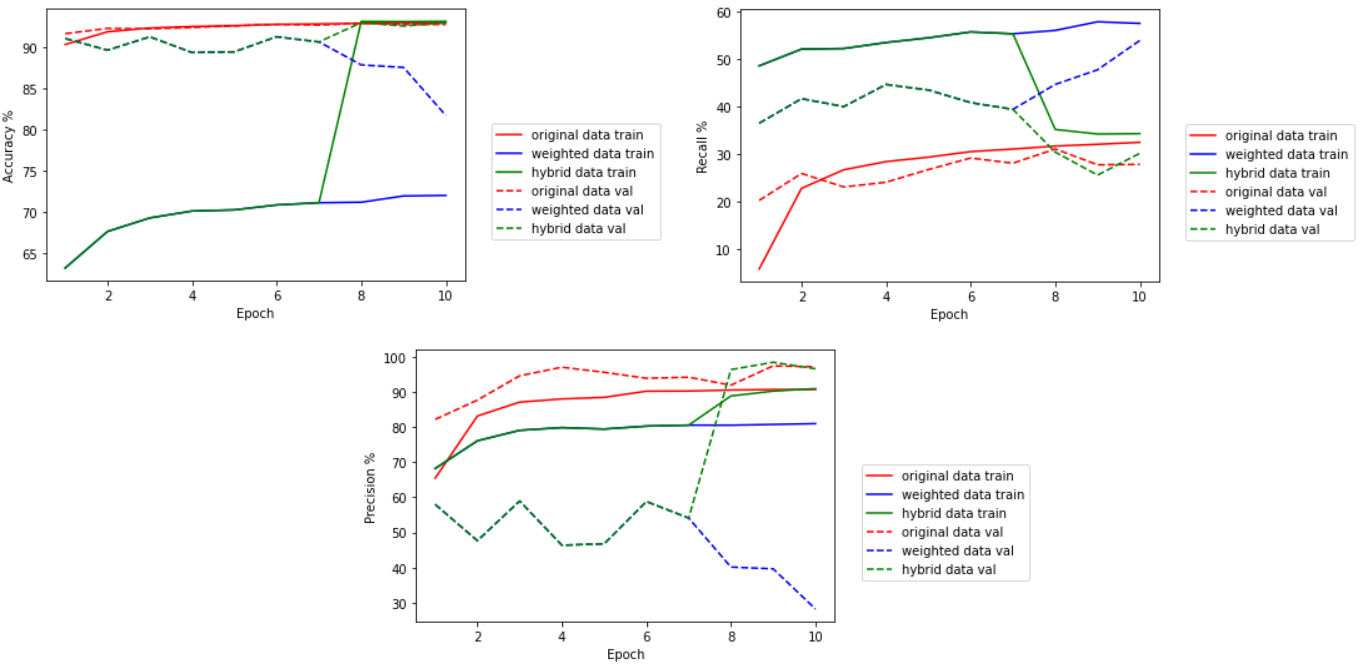
\includegraphics[width=0.9\textwidth]{metrics-acc-recall-prec.png}
\end{figure}
Das Training mit dem original Datensatz hat die höchste Accuracy, allerdings auch den geringsten Recall. Das liegt daran, dass das Modell fast nur darauf trainiert wird 0er Labels zu erkennen und hat daher zwar eine hohe Accuracy, dafür aber einen geringen Recall, da es die meisten 1er Labels nicht als solche interpretiert. Die Precision ist dafür aber wieder hoch. Ähnlich verhält es sich mit der hybriden Variante, allerdings ist der Recall etwas höher als bei der original Variante. Das liegt daran, dass überwiegend mit einem ausgeglichenem Datensatz trainiert wurde, wodurch das Modell mehr 1er Labels erkennt. Die gewichtete Variante hängt bei der Accuracy und Precision hinterher, dafür ist der Recall bei dieser Variante am höchsten, da ausschließlich mit einem augeglichenem Datensatz trainiert wurde. Außerdem ist auffällig dass die Metriken für die Validierungsdaten bei dem ausgeglichenen und hybriden Datensatz von den Metriken der Trainingsdaten abweichen, das hat den Grund dass die Validierungsdaten nicht an das Training angepasst wurden. Validierungsdaten sollten nie verändert werden und insbesondere nicht für das Training eingesetzt werden. Des Weiteren ist auffällig, dass das Training mit den ausgeglichenen Daten zwar eine recht hohe Accuracy und Recall liefert, allerdings ist auffällig, dass die Precision je mehr das Modell gelernt hat immer weiter sinkt. Das hängt unter anderem damit zusammen, dass der Recall immer weiter steigt und das Modell somit immer mehr 1er Labels als Signal interpretiert wobei viele davon gar keine Signale darstellen. Möglicherweise ist das Modell mit welchem trainiert wurde - efficientnet-b1 - nicht komplex genug um diese Aufgabe zu bewältigen. Das lässt sich auch recht gut aus den nächsten Diagrammen herauslesen:
\begin{figure}[h]
\centering
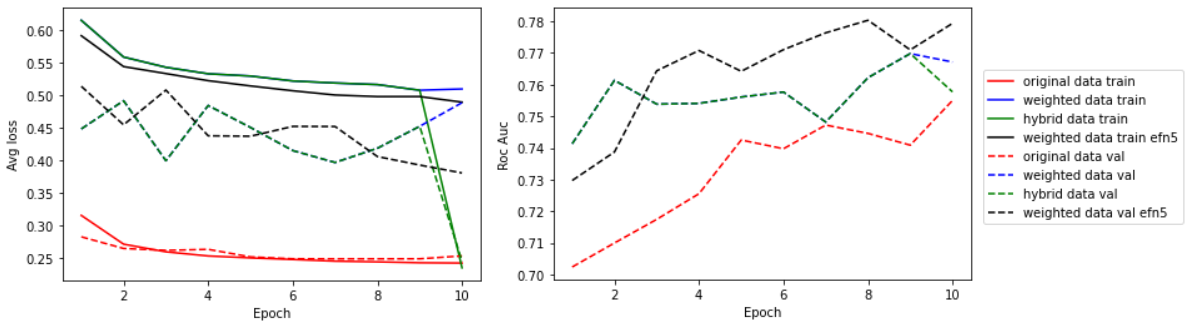
\includegraphics[width=0.9\textwidth]{metrics-avgloss-rocauc.png}
\end{figure}
Am interessantesten ist der Graph mit dem durchschnittlichen Loss. Sowohl bei der hybriden Variante als auch bei der original Variante ist der Loss recht niedrig gegen Ende der Epochen, während der Loss des Modells mit dem ausgeglichenen Datensatz auch am Ende noch recht hoch ist. Das hängt wie oben bereits erwähnt möglicherweise damit zusammen, dass das Modell nicht komplex genug ist. Da viele der Vorhersagen als Signal gesehen werden, allerdings viele der Vorhersagen falsch sind, ist der Loss entsprechend hoch. Der Roc/Auc Score ist bei allen Varianten gegen Ende fast gleich - der Score der gewichteten Variante ist am höchsten, da das Verhältnis von Recall und Precision besser ist.

TODO: stimmt diese Begründung über den Roc/Auc Score?

In den folgenden Diagrammen wurde das efficientnet-b5 genutzt, was einen komplexeren Aufbau als das efficientnet-b1 aufweist und dadurch möglicherweise die Problematik dieser Projektarbeit besser bewältigt.

TODO: Diagramme mit Metriken für efficientnet-b5

Abschließend kann man sagen, dass sowohl die Variante mit den original Daten als auch die Variante mit den gewichteten Daten beide Vor- und Nachteile haben. Daher ist die hybride Variante ein guter Kompromiss um die Vorteile beider Varianten auszunutzen. Allerdings muss man beim Oversampling aufgepassen, dass das Modell nicht übertrainiert wird auf die mehrfach genutzten Daten. Dabei kann uns Dataaugmentation weiterhelfen.

TODO: Referenz https://arxiv.org/abs/1710.05381

\section{Dataugmentation}
Gerade für die Strategie des Oversamplings ist es wichtig aufzupassen, dass das Modell nicht overfittet, also zu sehr auf spezielle Daten trainiert ist und somit auf allgemeinen Daten schlecht abschneidet. Da man beim Oversampling Daten mehrmals für dasselbe Training nutzt ist es sinnvoll die Daten etwas abzuändern, mithilfe von Dataaugmentation. Dabei geht es darum die Daten so zu transformieren, dass sie für das Training immer noch brauchbar sind, aber nicht mehr dem Original entsprechen. Dabei kann das Bild beispielsweise einfach horizontal oder vertikal gespiegelt werden. Es gibt noch viele weitere Möglichkeiten wie Rotieren, das Bild vergrößern und noch einige weitere. Diese Transformationen geschehen dabei zufällig, also mal wird beispielsweise nur horizontal gespiegelt, mal bleibt das Original erhalten, mal werden alle vorgegebenen Transformationen angewandt. Dadurch erhält man ein komplett neues Bild mit welchem das Modell trainieren kann ohne zu overfitten. Aber Dataaugmentation kann nicht nur sinnvoll sein, wenn man Oversampling angewandt hat, es kann auch sinnvoll sein wenn man ganz normale Trainingsdaten hat und das Modell möglichst breit gefächert auf den Daten lernen lassen möchte. Durch die Transformationen erhält man sozusagen alle möglichen weiteren Szenarien die das Modell erlernen kann.

TODO: Referenz Buch "Deep Learning mit Python und Keras von Francois Chollet"

\section{Scheduler}
Wenn das Modell trainiert wird, spielt die Lernrate eine große Rolle, wenn es darum geht die optimalen Parameter zu erhalten. Ist die Lernrate zu klein, dauert es lange bis der optimale Punkt erreicht ist, während bei einer zu hohen Lernrate dieser Punkt übersprungen werden könnte:
\begin{figure}[h]
\centering
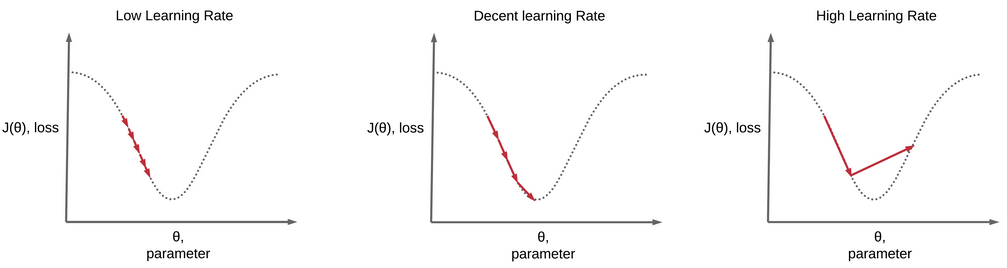
\includegraphics[width=0.9\textwidth]{lernrates-vs.png}
\end{figure}
Daher ist es wichtig eine gute Lernrate auszuwählen, welche somit unter die Kategorie der Hyperparameter fällt, mit welchen experimentiert werden muss bis man den optimalen Wert erhalten hat. Allerdings kann ein sogenannter Scheduler dabei Abhilfe schaffen. Die Grundidee des Schedulers ist die Lernrate über die Epochen hinweg zu verringern. Je höher die Epoche also je mehr man bereits trainiert hat, desto näher ist man am optimalen Punkt und die Lernrate muss immer weiter verringert werden um diesen Punkt nicht zu verpassen. Dadurch erhält man sowohl Vorteile einer hohen Lernrate als auch Vorteile einer geringen Lernrate: Anfangs ist die Lernrate noch hoch wodurch man sich dem Optimum schnell nähert, aber je näher man dem Optimum kommt desto geringer wird die Lernrate, wodurch man das Optimum nicht verpasst. Der Verlauf der Lernrate über mehrere Epochen hinweg könnte wie folgt aussehen:
\begin{figure}[h]
\centering
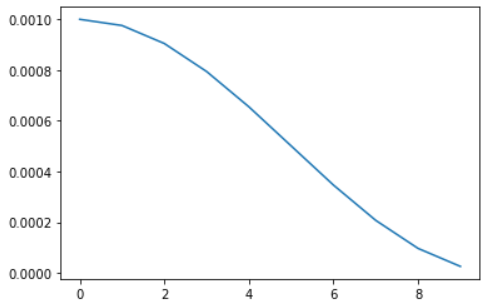
\includegraphics[width=0.9\textwidth]{lernrate-scheduler.png}
\end{figure}

TODO: Referenz https://www.deeplearningwizard.com/deep_learning/boosting_models_pytorch/lr_scheduling/

\section{K Fold Cross Validation}
Wenn man wissen möchte wie gut ein Modell trainiert ist kann man sich wie bereits weiter oben erwähnt bestimmte Metriken berechnen lassen die das Modell bewerten. Dabei kann es rein statistisch gesehen vorkommen, dass das Modell besonders schlecht repräsentative Trainingsdaten erhalten hat und somit auf realen Daten schlecht abschneidet. Um robuste Metriken zu berechnen hilft die K Fold Cross Validation. Dabei wird der gesamte Datensatz in k viele Teile unterteilt, wobei es entsprechend k viele Folds gibt. In jedem Fold wird das Modell neu trainiert, allerdings immer wieder mit anderen Trainings- und Validierungsdaten. Die Validierungsdaten beim ersten Fold sind beispielsweise der erste der k Teile, beim zweiten Fold der zweite und so weiter:
\begin{figure}[h]
\centering
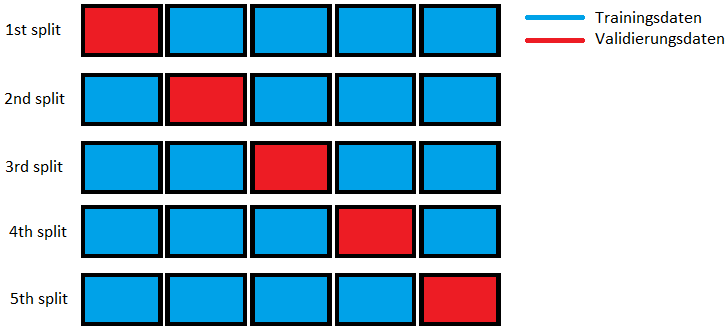
\includegraphics[width=0.9\textwidth]{folds.png}
\end{figure}
Die Metriken können nach Abschluss aller Folds gemittelt werden, wodurch man robuste Werte erhält. Außerdem kann ermittelt werden in welchem Fold das Modell am besten abgeschnitten hat. Wenn die einzelnen Parameterzustände der Modelle zwischen den Folds gespeichert werden, könnte man diese Parameterzustände beispielsweise für Vorhersagen auf echten Daten nutzen.

TODO: evtl irgendein Diagramm mit folds?
TODO: Referenz https://medium.com/dataseries/k-fold-cross-validation-with-pytorch-and-sklearn-d094aa00105f

\end{document}

